%!TEX root = constraint-layout.tex

% \newcommand{\teaserFigure}{
% 	\teaser{
% 		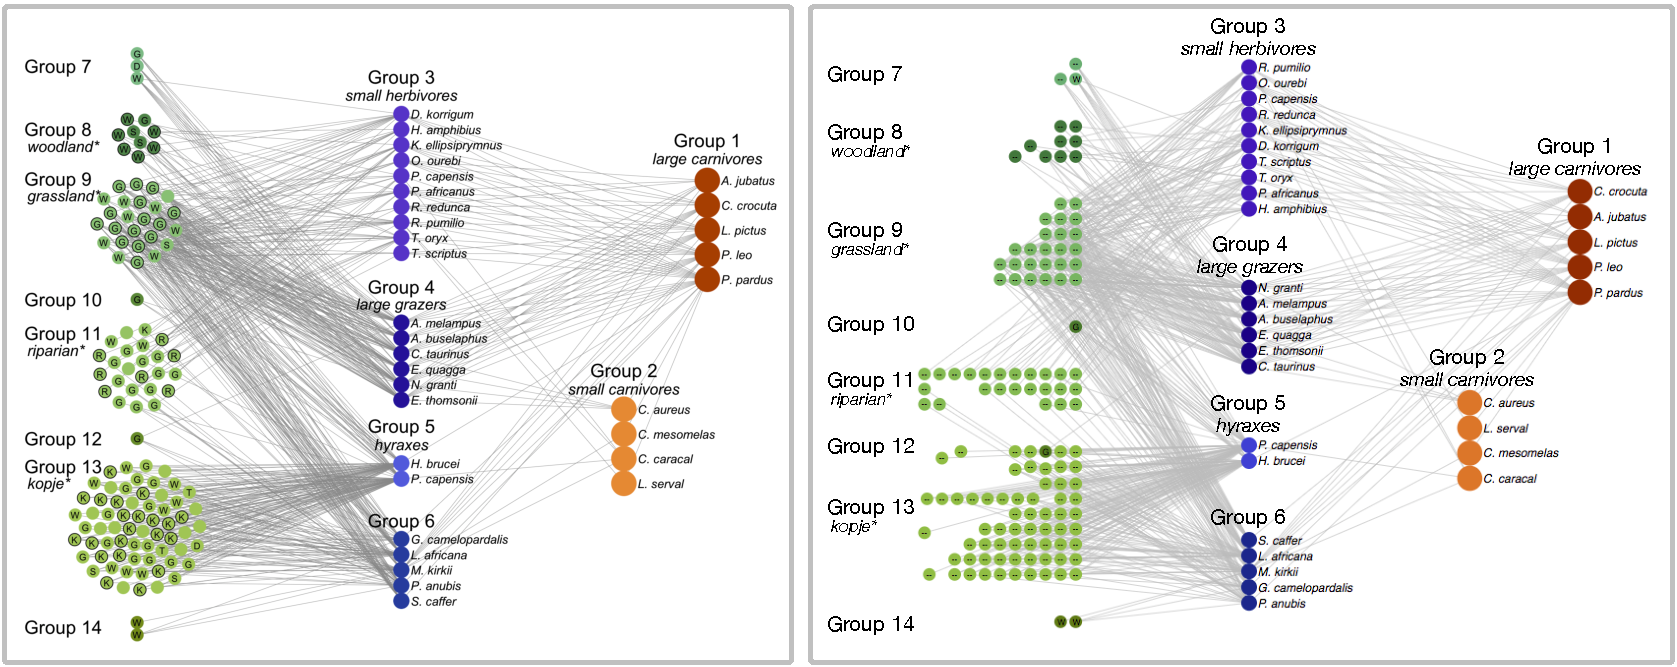
\includegraphics[width=\linewidth]{figures/serengeti-layout.pdf}
% 		\centering
% 	  \caption{\label{fig:teaser}}

% 	}
% }

\newcommand{\serengetiLayoutColumn}{
  \begin{figure}[t!]
    \centering
    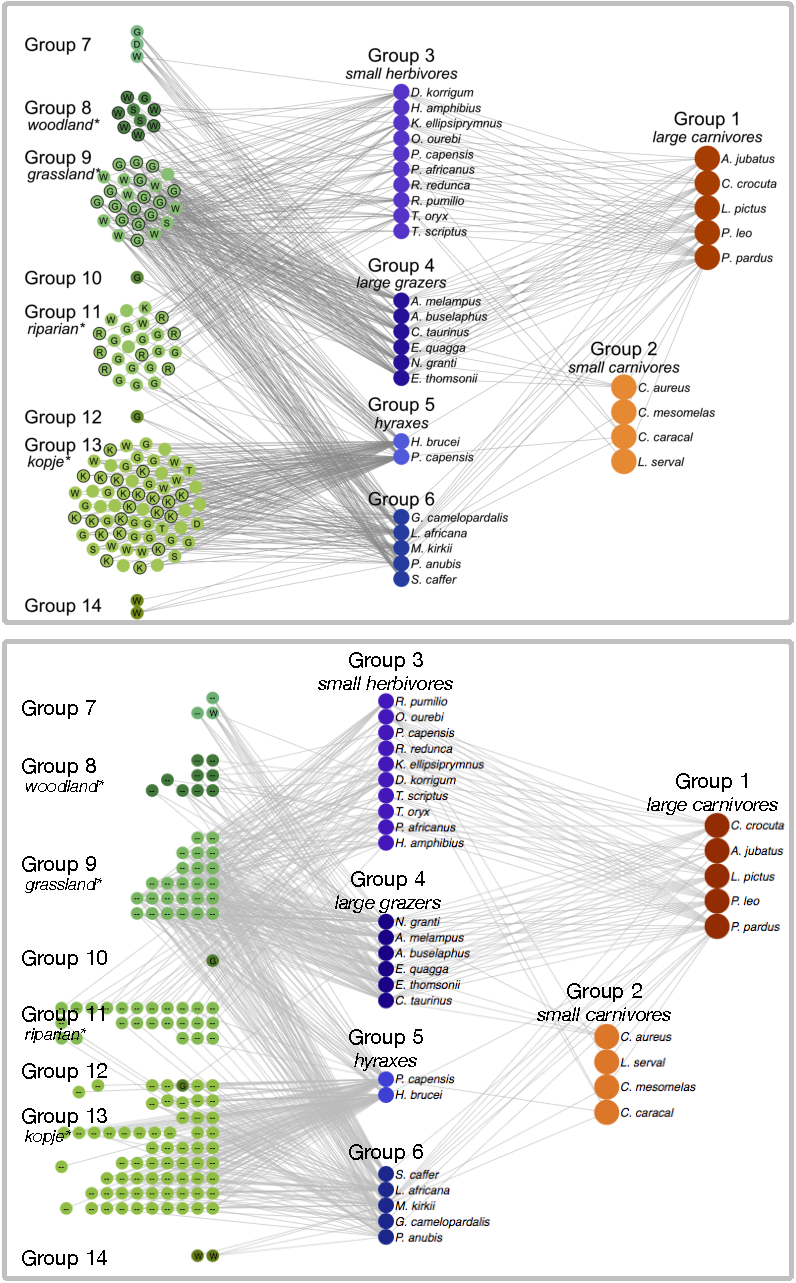
\includegraphics[width=0.81\columnwidth]{figures/serengeti-layout-column.pdf}
    {\caption{\label{fig:serengeti-layout}
    The layout for the Serengeti food web using our constraint language, as compared to Baskerville et al. \cite{baskerville2011spatial}.}}
    \vspace{-40px}
  \end{figure}
}

%%%%%%%%%%%%%%%%%%%%%%%%%%%%%%%%%%
%%%%%%%%% Demonstration %%%%%%%%%%
%%%%%%%%%%%%%%%%%%%%%%%%%%%%%%%%%%

\newcommand{\serengetiLayout}{
  \begin{figure*}[t]
    \centering
    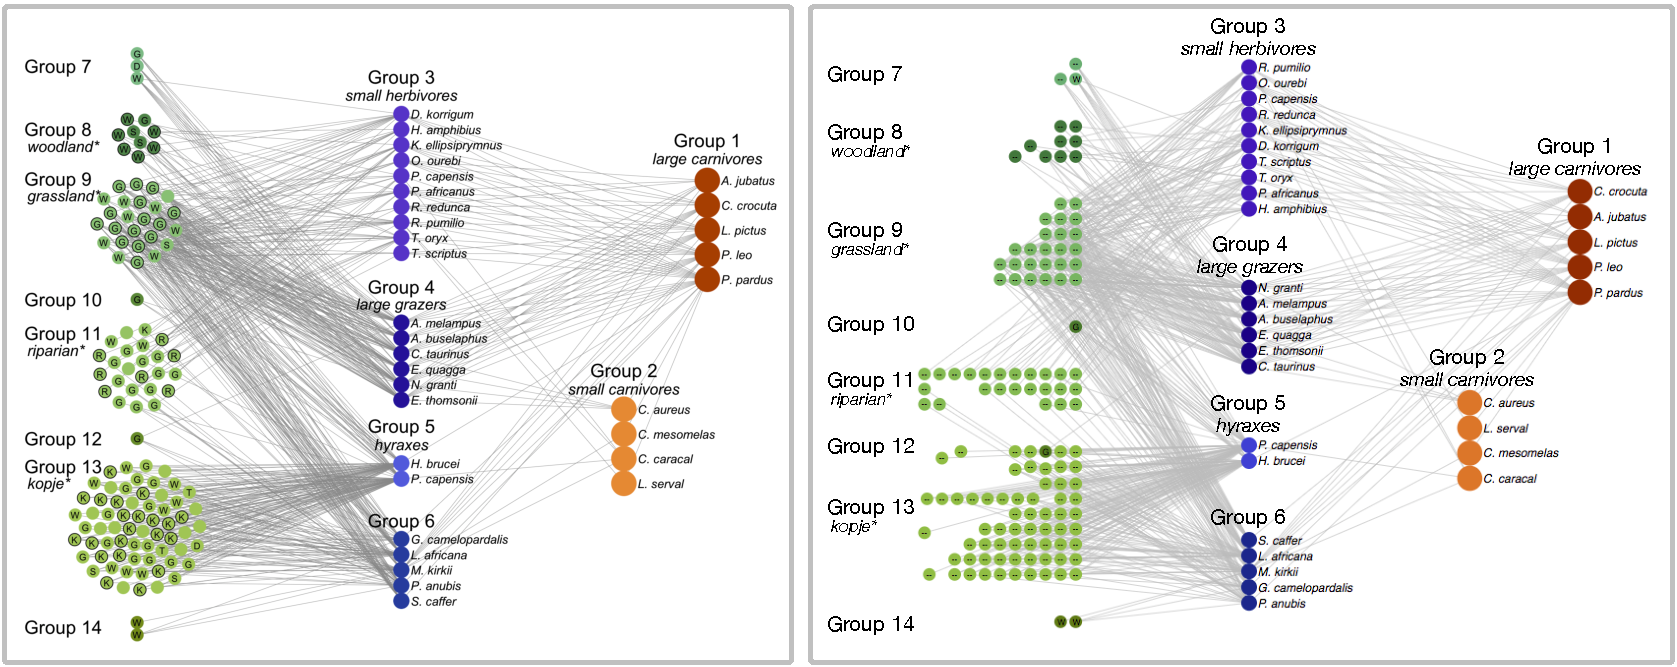
\includegraphics[width=\textwidth]{figures/serengeti-layout.pdf}
    \vspace{-20px}
    {\caption{\label{fig:serengeti-layout}
    The layout for the Serengeti food web using our constraint language, as compared to Baskerville et al. \cite{baskerville2011spatial}. \todo{retake photos on retina screen} \todo{label the two sides of the figure a/b}}}
  \end{figure*}
}

\newcommand{\serengetiSpec}{
  \begin{figure}[t]
    \centering
    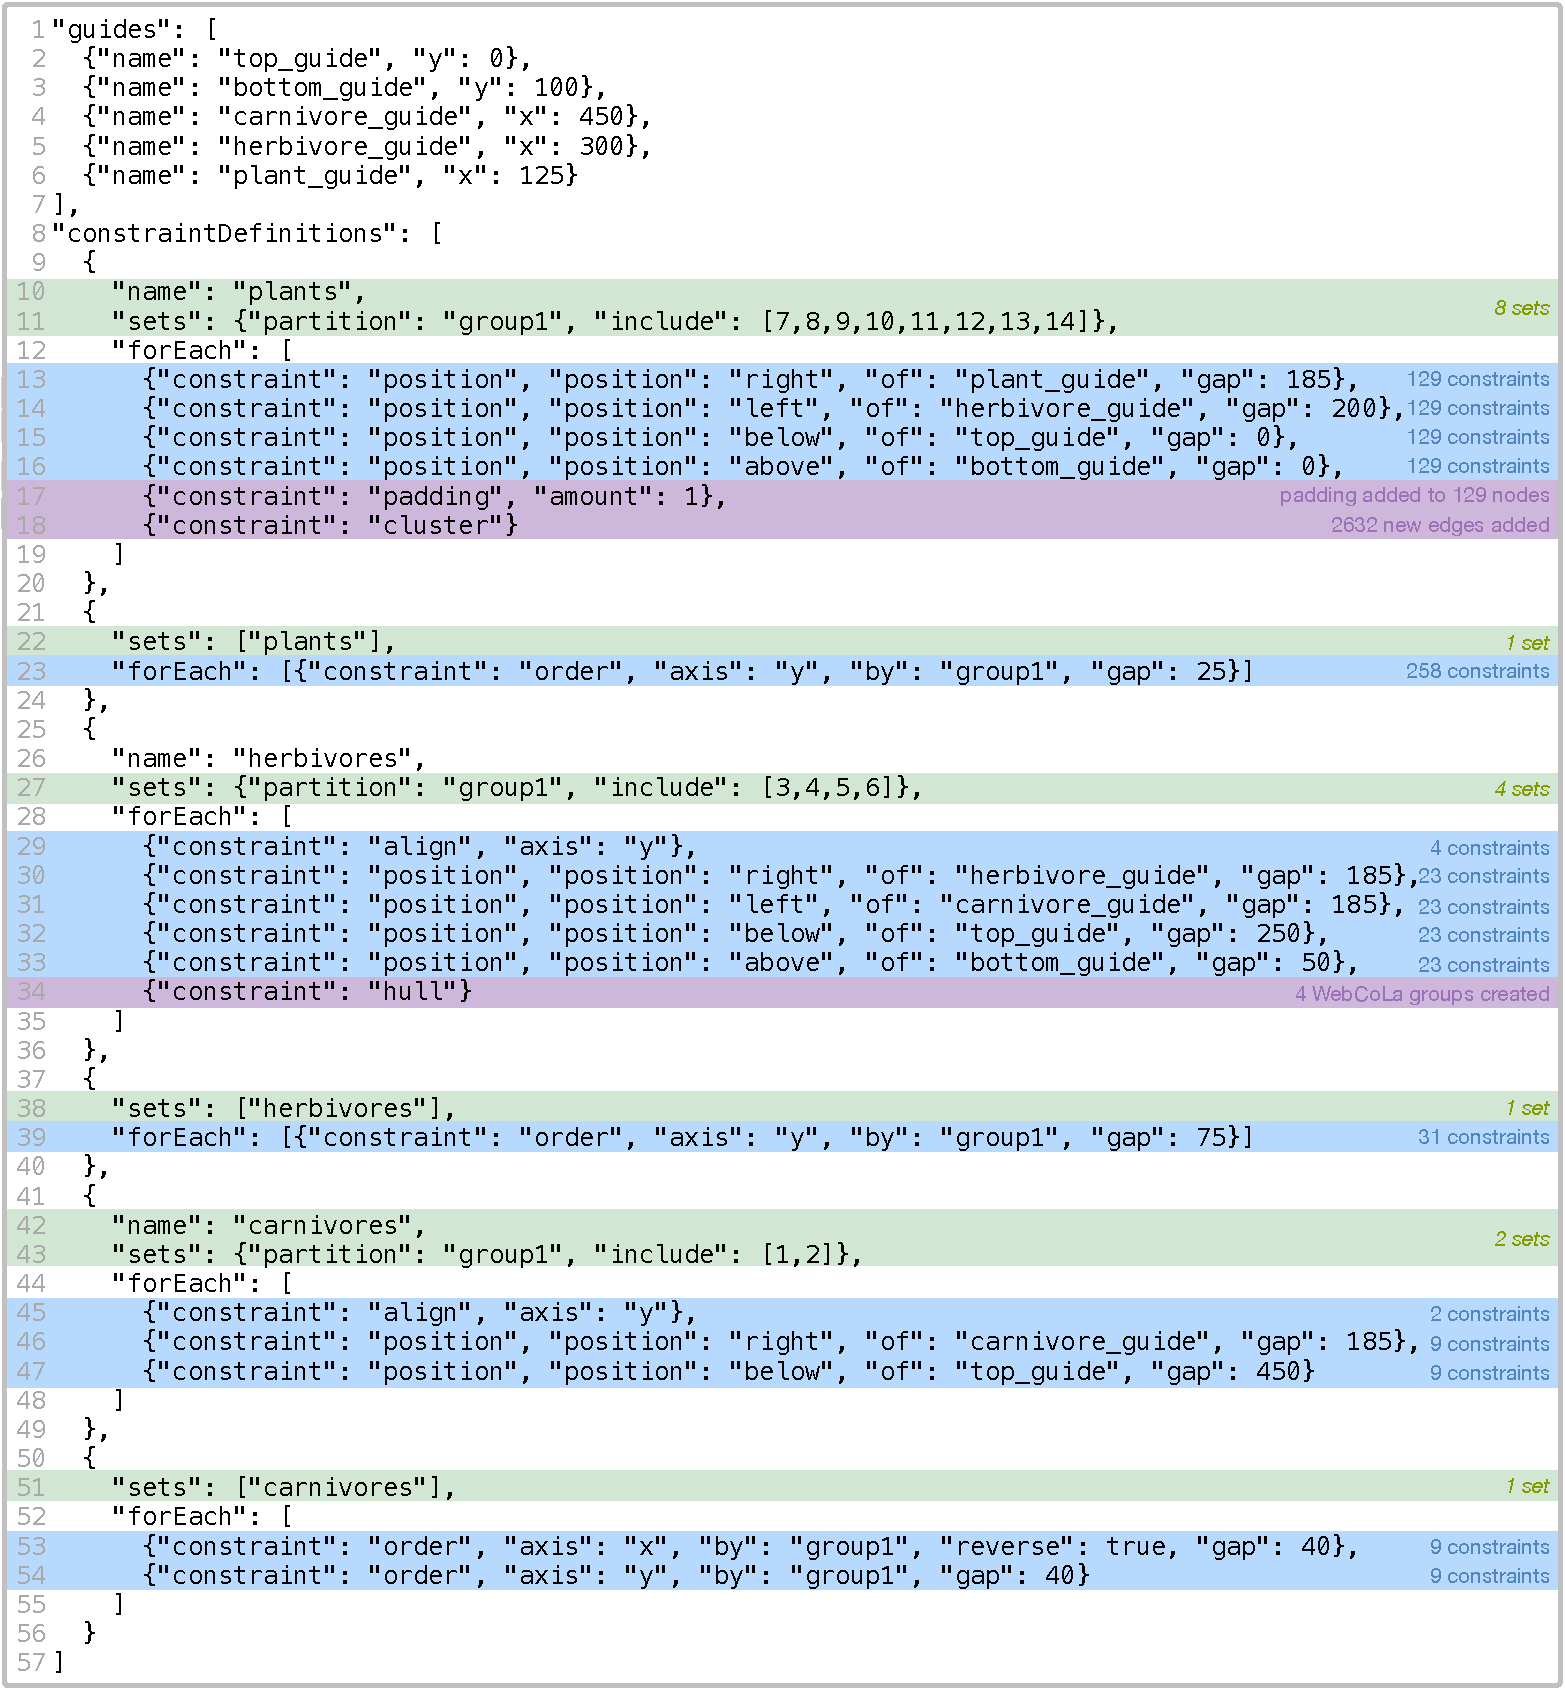
\includegraphics[width=\columnwidth]{figures/serengeti-spec.pdf}
    \vspace{-20px}
    {\caption{\label{fig:serengeti-spec}
    The \projectname~specification for the Serengeti food web shown in Figure~\ref{fig:serengeti-layout}. The code is annotated with the number of sets produced, the number of edges added, and the number of WebCoLa constraints generated for the final layout.}}
  \end{figure}
}

\newcommand{\syphilisLayout}{
  \begin{figure*}[t]
    \centering
    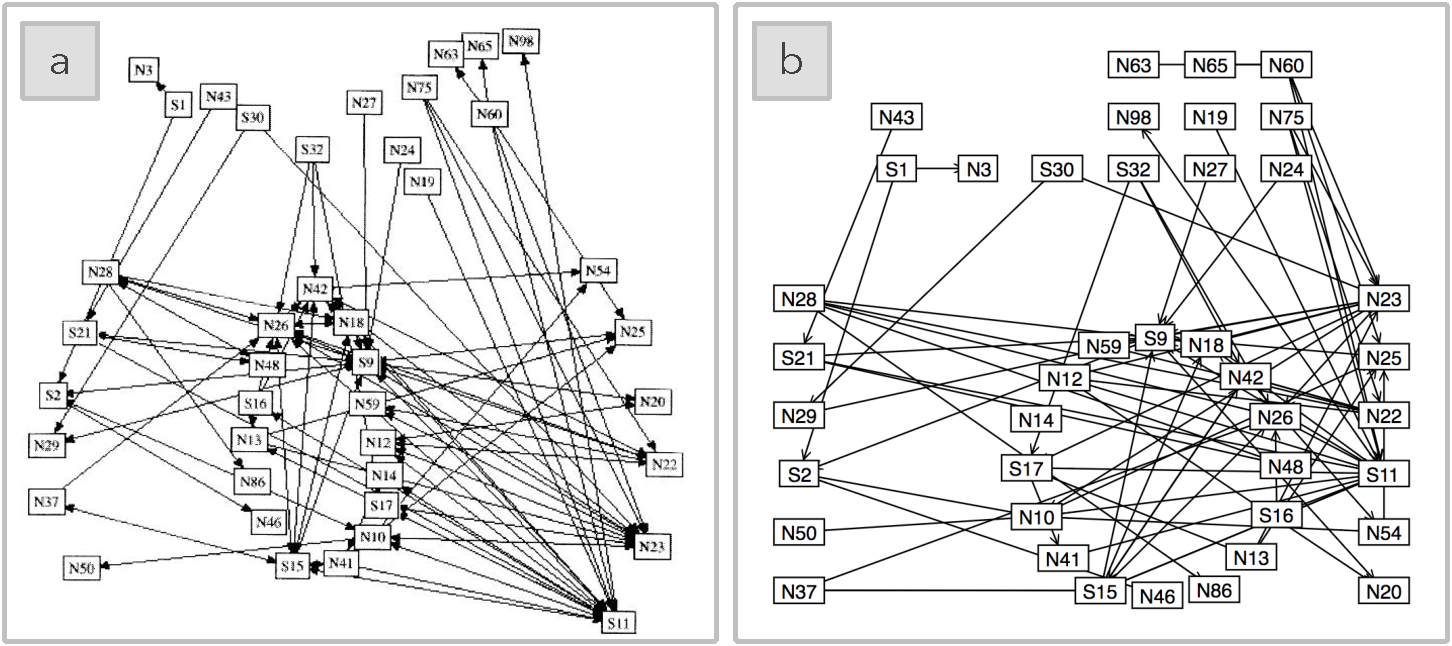
\includegraphics[width=\textwidth]{figures/syphilis-layout.pdf}
    \vspace{-20px}
    {\caption{\label{fig:syphilis-layout}
    The layout for the syphilis social network from (a) Rothenberg et al. \cite{rothenberg1998using} as compared to (b) the \projectname~layout.}}
  \end{figure*}
}

\newcommand{\syphilisSpec}{
  \begin{figure}[t]
    \centering
    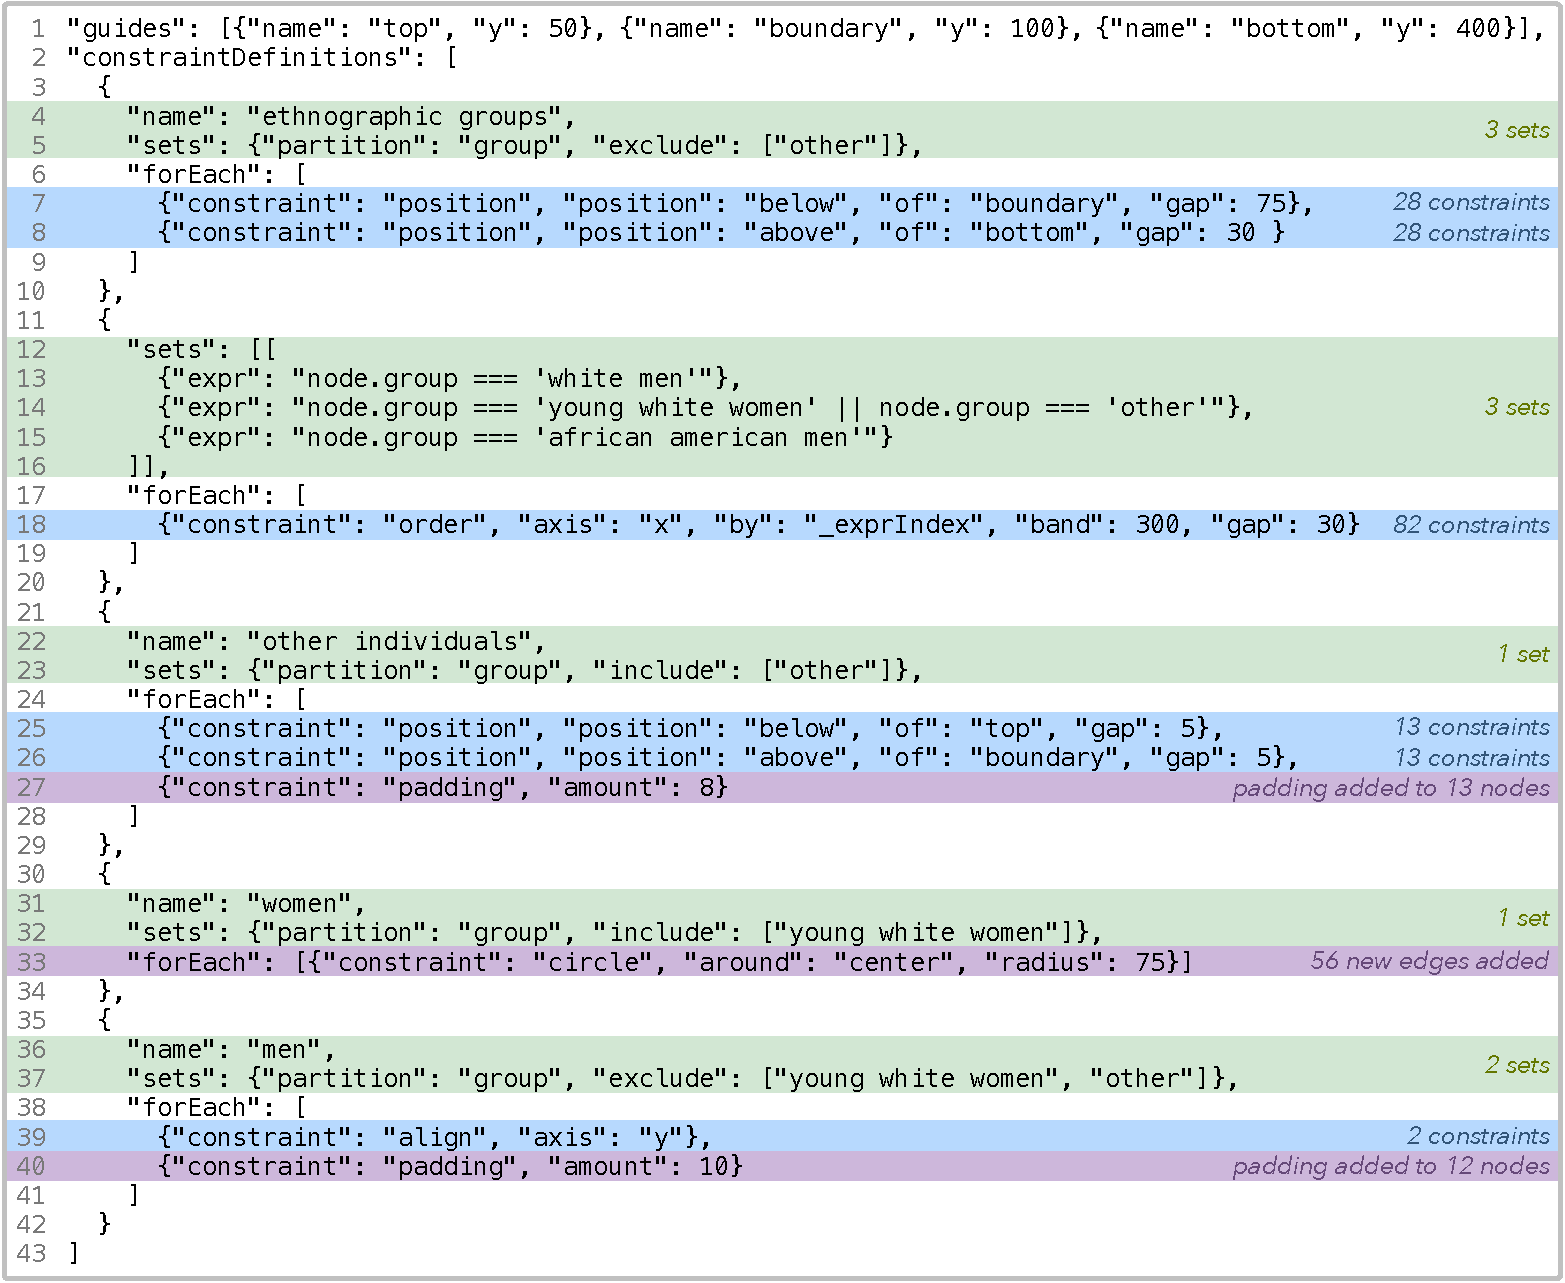
\includegraphics[width=\columnwidth]{figures/syphilis-spec.pdf}
    \vspace{-20px}
    {\caption{\label{fig:syphilis-spec}
    The \projectname~specification for the syphilis social network shown in Figure~\ref{fig:syphilis-layout}. The code is annotated with the number of sets produced, the number of edges added, and the number of WebCoLa constraints generated for the final layout.}}
  \end{figure}
}